\chapter{Design}

As the final prototype will utilise intermixing to affect a behaviour, two different prototypes will have to created. One that is overloaded with the message (75 percent) and one that is intermixed (45 percent). The following chapter will explain how the design came to be and the decisions that affected the final design.

\section{Final design; Drive Through}
The design is initially based on the design requirements found in section 2.6. Here, it is established that the prototype will be a virtual reality (VR) installation. For the VR installation to attempt to incite a behavior change through the concept of intermixing, several factors are considered.

A non-functional requirement states that the issue presented must feel near and personal to lower the distance barrier. As the target group is people living in Denmark, the prototype should attempt to resemble a Danish environment. As it was discovered in the State of the art, section 2.4, exaggerated feedback has a positive effect on the user, and thus it was decided to mix this into the design and present a shifting environment, this will be explained further in the sub-section “The Environment” below. In order to present a shifting environment, it was decided to place the user in a vessel, that moves through terrain; for this specific purpose, a self-driving car was chosen.
A car allows the user access to a front seat with a view over the environment, while having it self-driving allows the user to focus on the environment instead of physically driving the vehicle, as seen in picture XX below. The car will follow a straight road, as the environment around the user gets presented to them. 

 \begin{figure}[H]
        	\centering
        	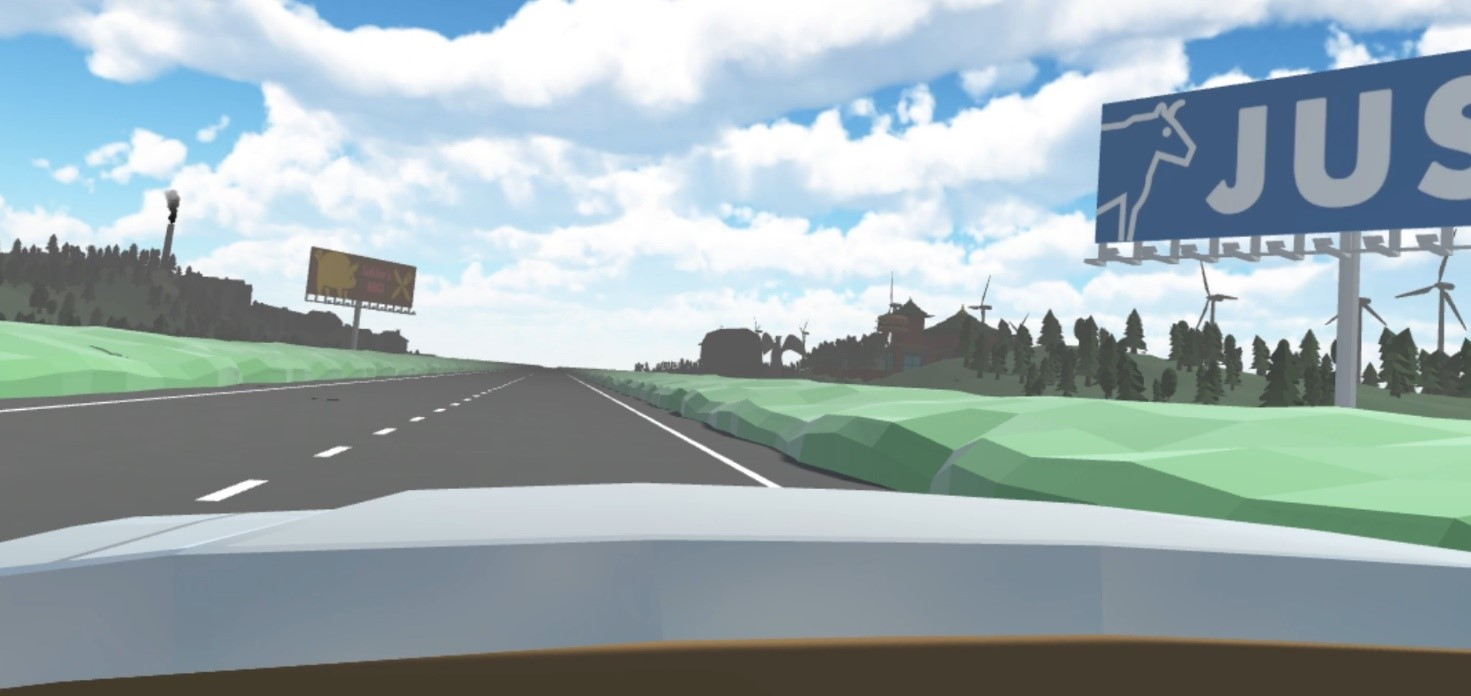
\includegraphics[width=0.9\linewidth]{figure/Design/Designpic1.jpg}
        	\caption{Picture displaying the view from the car in the prototype}
        	\label{fig:designpic1}
        \end{figure}
        
        
 The story of the prototype will get told through a mix of two things; the environment around the user, and the radio within the car. This allow for additional immersion within the VR experience, as well as a way for the strategy of intermixing to affect the number of objects in the environment, and the amount of news on the radio that are relevant for the issue at hand, in this case meat consumption. How these are divided are explained further in the sub-chapter “The Environment”.

Another requirement states that the user should have opportunities for consistent and visible actions, in order to reduce dissonance. This means that there must be an interaction within the car, that the user can engage. This was taken as an opportunity to give the user an action that could be measured and was relevant to the topic of the issue. As VR makes small, novelty interactions fun (Reference?), it was decided to place a button in front of the user in a car. This button produces a burger, that is presented for the user to eat. If the user interacts with the burger, and places it close to the mouth, the burger will appear to get eaten by the user. The prototype then measures the number of burgers produced during the duration of the experiment, which allows to see if the narration of the radio or the objects in the environment directly affects the users during the experiment. The burger itself directly relates to meat consumption and will be explained to the user over the narrative element of the installation. 

 \begin{figure}[H]
        	\centering
        	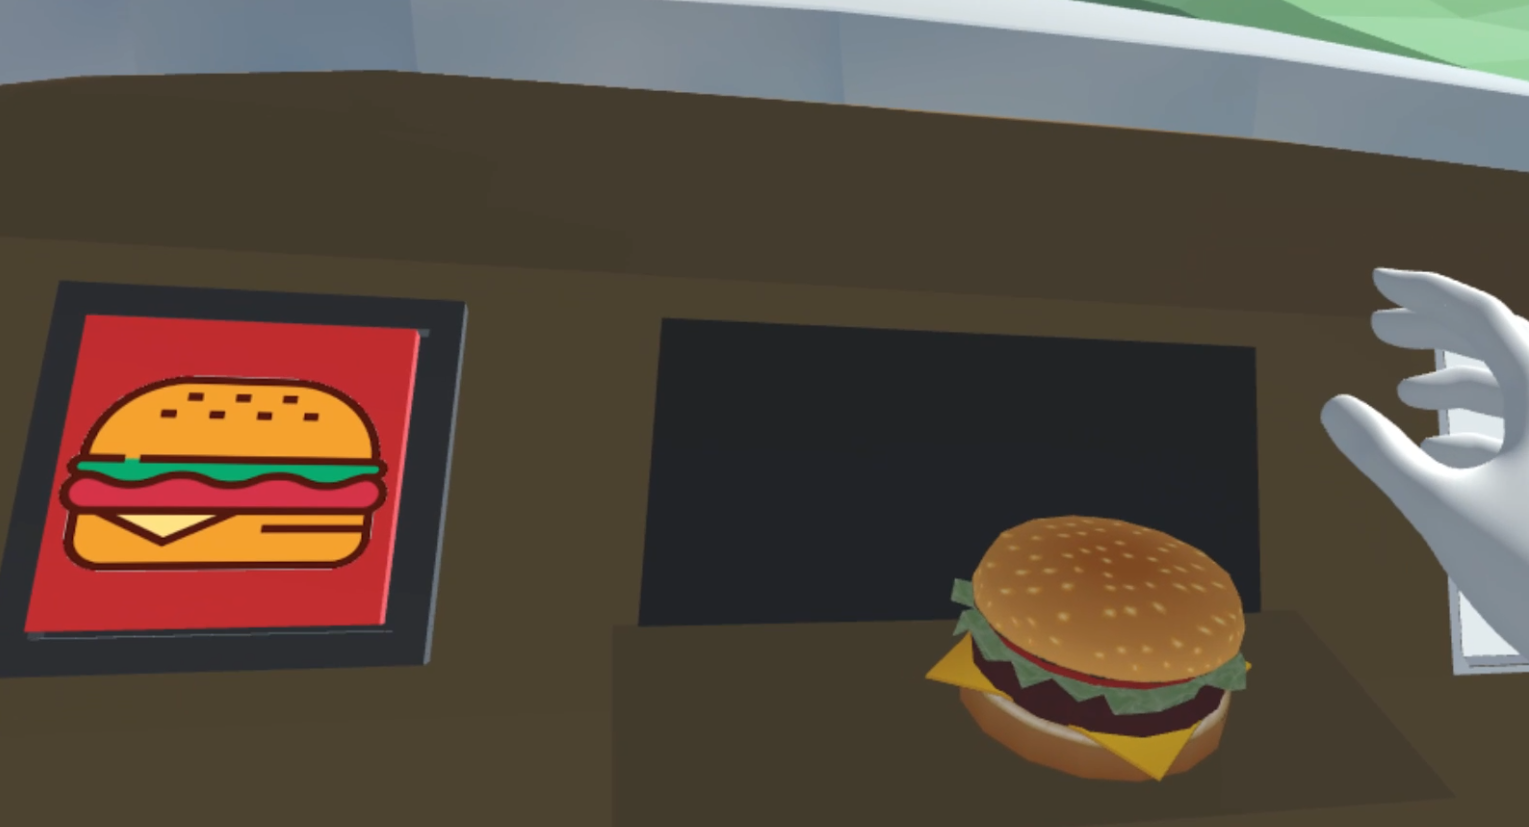
\includegraphics[width=0.9\linewidth]{figure/Design/Designpic2.png}
        	\caption{Picture displaying the interaction with the burger}
        	\label{fig:designpic2}
        \end{figure}


\subsection{Graphics}
The graphical expression of the prototype must be non-realistic, as found in the design requirements in section 2.6. Having the prototype in a non-realistic VR setting also makes sure that the issue is not communicated forthright and avoids inciting fear, by mixing in unrealistic or silly actions. The following Picture XX shows the graphical expression, with an emphasis on a cartoon-like art style. It also displays a humorous take on the happenings along the road in the environment; a chicken farm slaughtering chickens in a shredder.

 \begin{figure}[H]
        	\centering
        	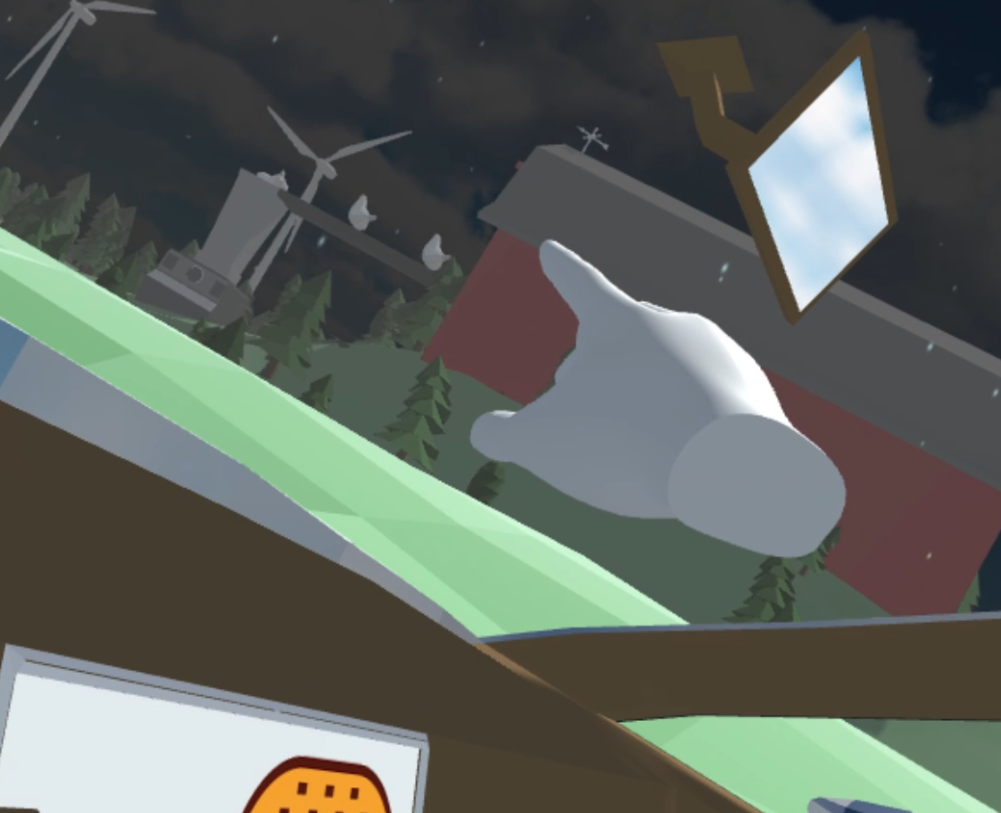
\includegraphics[width=0.9\linewidth]{figure/Design/Designpic3.png}
        	\caption{An example of a humorous object in the environment, displayed in the cartoon-like graphics style}
        	\label{fig:designpic3}
        \end{figure}
\subsection{Environment and Narration}
The process on the experiment is linear, as it starts with the user driving in the front seat of a moving car. As the experience progresses, objects will be a long the road for the user to observe. Meanwhile, the radio will contribute with different news stories, the

 \begin{figure}[H]
        	\centering
        	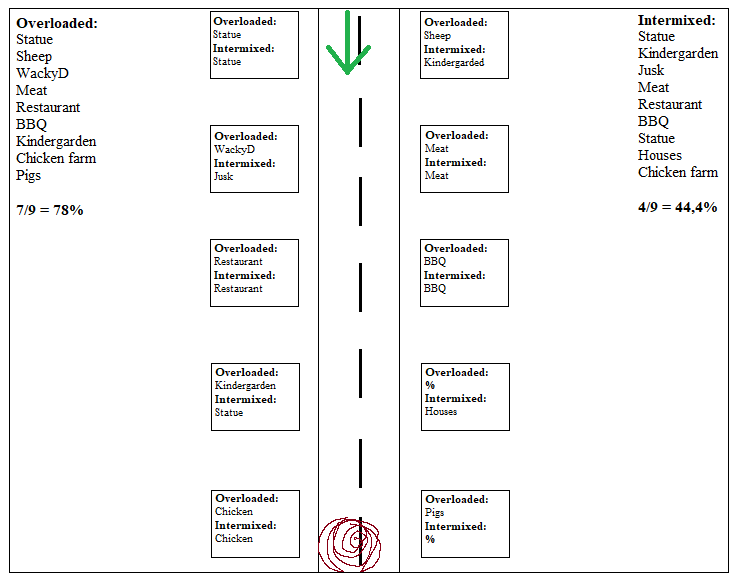
\includegraphics[width=0.9\linewidth]{figure/Design/Designpic4.png}
        	\caption{An overview of the objects placed in the environment}
        	\label{fig:designpic4}
        \end{figure}


\section{Usability test}
    For discerning the usability of the interactions in the design, a simple test using the SUS scale questionnaire, was conducted. The test participant were told to put the Virtual Reality headset on their head, and got one controller handed to their primary hand. The participant were observed during the test, and afterwards instructed to fill out the SUS questionnaire.
    
\subsection{Test setup}
    The setup for the Usability test (seen in \autoref{fig:usabilitySetup}), using the SUS questionnaire, where the test subject, going through the test, were positioned in front of the monitor with the HMD on. The observer seated nearby, were noting any miscellaneous usability related things.
    
\begin{figure}[H]
    \centering
    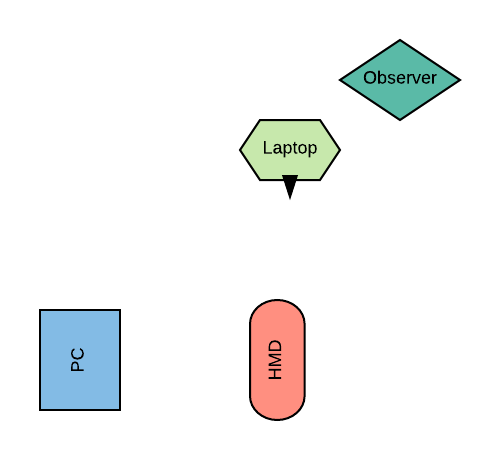
\includegraphics[width=0.6\linewidth]{figure/Design/UsabilitySetup.png}
    \caption{The setup of the usability test, with the \color{red}{HMD/User}, \color{blue}{PC}, \color{teal}{Observer}, and \color{green}{Laptop for SUS}}
    \label{fig:usabilitySetup}
\end{figure}

\subsection{Test results}
After the test participants have answered all 10 questions on the SUS questionnaire, the SUS score that values the usability of the design, is calculated using the official SUS method\cite{SUS}. For all odd numbered questions (1, 3, 5, 7, and 9,) 1 is subtracted from the score. For all even numbered questions (2, 4, 6, and 8,) the scores are subtracted from 5, this results in the all question scores being between the range of 0 and 4. These new scores are summed up and multiplied by 2.5, resulting in a number between 0 and 100\cite{SUS}. The final numbers' mean resulted in a mean of 87, which in SUS terms, means that the usability of the design is rated at excellent\cite{SUS}. All the individual calculated SUS scores and their reference points can be seen in \autoref{fig:susplot}. 

    \begin{figure}[H]
        \centering
        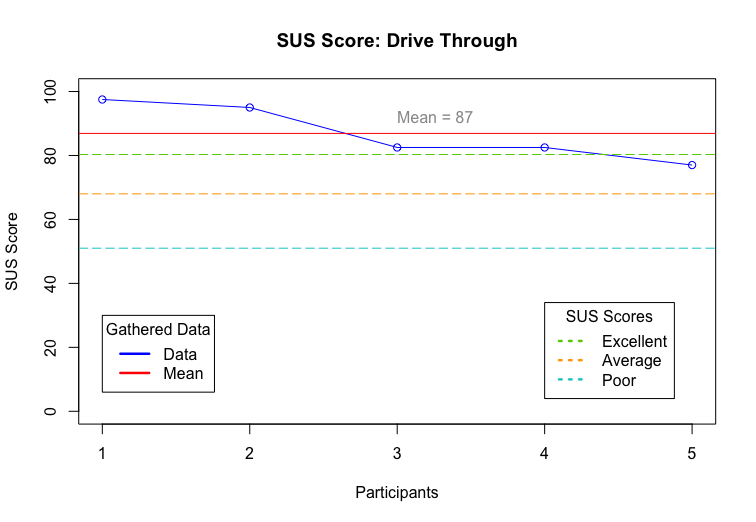
\includegraphics[width=0.8\linewidth]{figure/Design/susplot.png}
        \caption{SUS plot showing the calculated SUS score for each participant. With a total of mean of 87, the score is above the threshold that is stated to be an excellent SUS score.}
        \label{fig:susplot}
    \end{figure}

\subsection{Observations}
    During the usability test, an observer noted any usability issues that would occur. These notes correlated into the issue that $\frac{4}{5}$ test participants initially did not press the correct trigger on the Oculus touch controller when grabbing for the burger, and then being confused about how to grab the burger. Eventually $\frac{5}{5}$ users figured out that the controller had two trigger buttons, and then proceeded to expectedly grab the burger and quite naturally move it towards their mouth and eat it. This button was changed to the button that most test participants found natural to press to grab the burger. It was also noted that $\frac{5}{5}$ test participants smiled when the natural reaction to eat the burger, and outcome of eating the burger in Virtual Reality connected.
    
\section{Design summary}
